\documentclass[main.tex]{subfiles}
\ProvidesPackage{preamble}

\usepackage[nottoc]{tocbibind}
\usepackage[english]{babel}
\usepackage[utf8]{inputenc}
\usepackage[table]{xcolor}
\usepackage[nohead, nomarginpar, margin=1in, foot=.25in]{geometry}
\usepackage{tabularx}
\usepackage{graphicx}
\usepackage{float}
\usepackage[english]{babel}
\usepackage{paralist}
\usepackage{datetime}
\usepackage{afterpage}

\begin{document}

\section{Design}

\subsection{General Design Decisions}
We have chosen pandas dataframes \cite{pandas} as the common data format for both data exchange and any calculations. Pandas provides us with data structures ``that cohere with the rest of the scientific Python stack`` \cite{mckinney2011pandas}, such as NumPy, which we are using to calculate historical returns and risk metrics (\ref{BL Structure}). Additionally, it is supported natively by many third party APIs and can even be used to read data from SQL databases. For additional information, please consult the official pandas documentation \cite{pandas}.

\subsection{Overview of System Architecture}

Before discussing any specific component and architectural layer in depth, it is worth revisiting our original architecture \cite{TR}.
\begin{figure}[H]
    \caption{Original Thalia System Architecture \cite{TR}}
	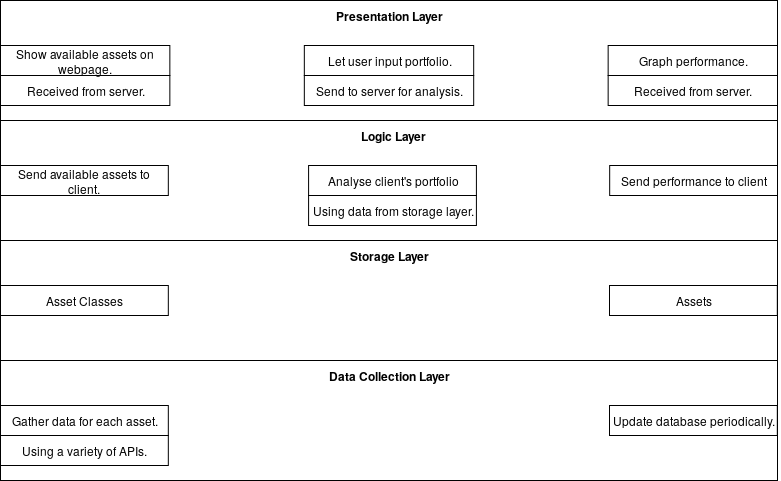
\includegraphics[width=\textwidth]{04Design/04Pictures/architecture_layer_diagram.png}
\end{figure}
The above schematic illustrates how we modified a typical Three Layer architecture [citation needed] to include a Data Collection Layer. Subsequent discussion will refer to this layer as the `Data Harvester`. It consists of adapters for third party APIs which offer price data for financial assets. The associated API will be queried according to a configurable interval to allow for live updates to our price data. Additionally, initial seeding of the database with historical price data can also be achieved via the Data Harvester. The decision to isolate this system component has been made in order to increase security by limiting the acess of the Thalia web service to the financial data database to read-only and to allow for independent scaling of the Data Harvester and our web service \cite{TR}.

While the architecture of our system has stayed the same, there have been some modifications to individual components. Most notable are the changes to the Database Structure examined in \ref{DB Structure}. The following sections will provide for a discussion of design decisions made on a layer-by-layer basis.

\subsection{GUI Structure}

% TBD

\subsection{Business Logic Structure}
\label{BL Structure}

The responsibility of our business logic can be summarised as follows: Given an investment strategy specification input from a user via the GUI, retrieve relevant financial data from the database to perform calculations for the historical performance and associated risk metrics.

To achieve this, we have developed a library (Anda) that performs the necessary calculations. Anda is decoupled from both the presentation and database layer by relying on external providers for any price data and the specification of a strategy.
This decision has been made to allow for alternative sources of price data in the future. One of our optional features for future development is allowing users to input their own price data for assets not supported by Thalia. This data could be uploaded, for example, as a CSV file or JSON. Without our current design, i.e. by coupling calculation of performance and metrics to database access, we would have to modify the business logic to support multiple data sources. Given our current implementation, however, we can simply parse the user data into a pandas dataframe in a wrapper around Anda and then call functions within the library as require.
Currently supported metrics include Total Return, Max Drawdown, Best / Worst Year, and the Sharpe and Sortino Ratios. However, the library is open for extension, hence additional metrics may be added at any point.

For a closer look at how an investment strategy is specified, consider the following class that serves as input to Anda library functionality (e.g. for calculating the Sharpe Ratio [citation needed]):

\begin{lstlisting}[language=Python, caption=setup.py - Development environment, label=lst:Development_env]
import pandas as pd

class Strategy:
    def __init__(
        self,
        start_date: date,
        end_date: date,
        starting_balance: Decimal,
        assets: [Asset],
        contribution_dates,  # implements __contains__ for date
        contribution_amount: Decimal,
        rebalancing_dates,  # implements __contains__ for date
    ):
        self.dates = pd.date_range(start_date, end_date, freq="D")
        self.starting_balance = starting_balance
        self.assets = assets
        self.contribution_dates = contribution_dates
        self.contribution_amount = contribution_amount
        self.rebalancing_dates = rebalancing_dates
\end{lstlisting}

Here, Asset is a simple dataclass consisting of a ticker string (e.g. `MSFT` for Microsoft), a weight as a share of the portfolio overall (e.g. 0.25), a pandas dataframe holding historical price data ordered by date, and a pandas dataframe for dividends data (if any).

As alluded to earlier, functions within the library depend on a Strategy object for their calculations. For example:

\begin{lstlisting}[language=Python, caption=setup.py - Development environment, label=lst:Development_env]
def total_return(strat) -> pd.Series:
\end{lstlisting}
will calculate a series of total return values ordered by date within the date range specified in the passed Strategy instance.

Another important design decision has been the choice of data type to represent money, for example for price data. For this, we have chosen the Decimal type from the Python Standard Library decimal module, since it ``provides support for fast correctly-rounded decimal floating point arithmetic`` \cite{PyDecimal}. As rounding errors and imprecision are unacceptable for our application, using the Decimal type will allow us to reliably compute figures for prices, risk metrics, etc.

Finally, we have chosen NumPy \cite{walt2011numpy} for performing numerical calculations as this allows for highly optimized computation through the use of vectorized operations.

\subsection{Data Harvester Structure}
The role of Data Harvester is collecting live data from multiple source  refining it in a format that makes it usable by Anda and easily storable  by our in house DBMS system Finda. In addition to this a mechanism for changing the data collected and adapting to the market demands has to exist. Another requirement relates to the limitations that imposed by the APIs used. 



\subsubsection{Continuous Updating Mechanism}
The Updating is comprised of 3 components:
\begin{itemize}
    \item \textbf{The update procedure} made out of a series of methods. The procedure starts by looking at what APIs are available to be called. Each API has a update list that contains the tickers of the financial assets that we wish to get data on and the last and earliest record we have on that asset. If it is the first time when asking for data on a specific asset then we ask for all data available between 1970/1/1 up until the last financial day available. If the number of allowed calls for a API is greater then the number of assets to be updated then all assets can be updated in a daily run. However if it is not possible to update all assets in one update run then will update the rest of the assets in the following run so that we can get as close as we can to live data. In order to have a better view of this a flow chart of how the 
    \item \textbf{A run\_updates script} that starts an update round. It contains the configuration with the API names, the location of the access key (if it exists) and the number of calls to be done for each API. 
    \item \textbf{An initialiser} module that is based on the persistent data folder that contains the asset classes and the assets in the form of CSV files. The initialiser gets a configuration similar to that given to the run\_updates script. Based on the asset classes, the assets and the APIs given, the initialiser creates an update\_list for each API.
\end{itemize}

\begin{figure}[H]
    \centering
    \caption{Data Harvester Update round\cite{TR}}
	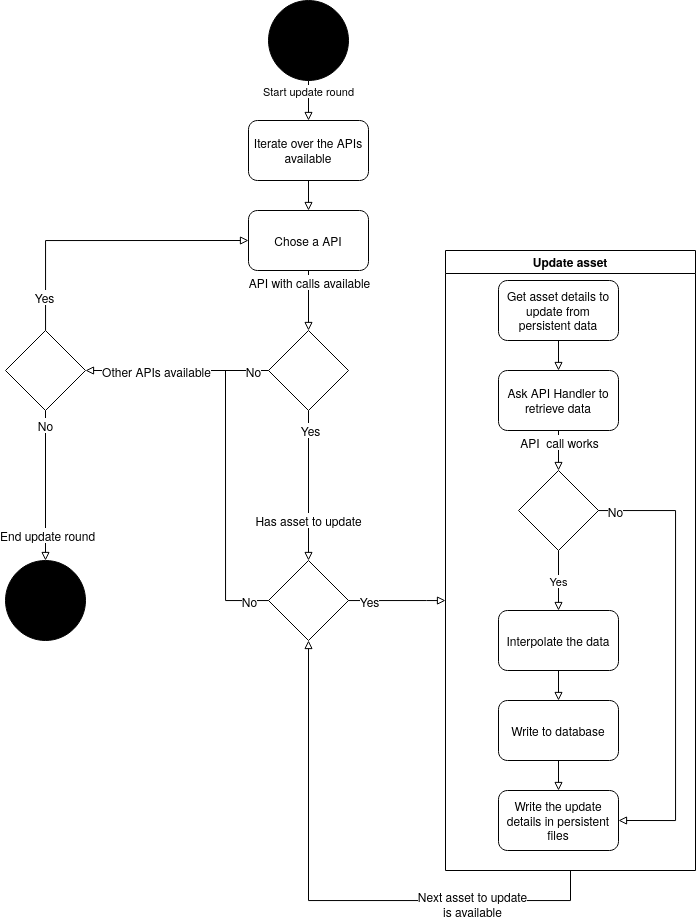
\includegraphics[width=0.7\textwidth]{04Design/04Pictures/update_mechanism_flow_chart.png}
\end{figure}

In order to know more about how the updating mechanism works consult the logs section in Maintenance design.


\subsubsection{APIs Handler}
For each API, the API Handler has a call method and a method that formats the data so that it fits our data model. In addition, there also is an api\_selector method that makes the right API call based on what asset class is requested and a dataframe format checker that does a final check before sending the data to the updating mechanism. 


\begin{figure}[H]
    \centering
    \caption{API Handler Flow Chart\cite{TR}}
	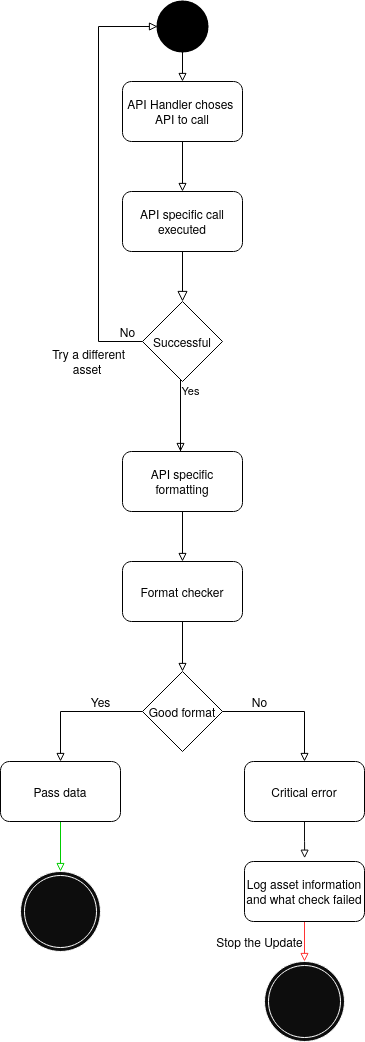
\includegraphics[width=0.47\textwidth]{04Design/04Pictures/api_handler_v2.png}
\end{figure}

\subsubsection{Interpolation}
Our business logic library requires continuous data in order o be able to perform the numerical analysis. In order to transform real life data that includes weekends and bank holidays into a continuous data sets we have used interpolation. The type of interpolation used is nearest neighbour. To be more precises, the algorithm designed goes over the data in pairs of adjacent dates, if there are any missing days then the older nearest neighbour is duplicated over the missing days. In addition to this the duplicated rows are flagged as interpolated in the database. Here is a example of how it would look like:
\textbf{\newline Pre-Interpolation: }
\begin{center}
 \begin{tabular}{||c c c c c c c c||} 
 \hline
 Index & ADate & AHigh & ALow & AOpen &A Close&AssetTicker&IsInterpolated\\ [0.5ex] 
 \hline\hline
 3&2000-11-16&126.86&126.89&126.86&87.36&VFIAX&0 \\ 
 \hline
 4&2000-11-17&126.44&126.44&126.44&87.07&VFIAX&0\\
 \hline
 5&2000-11-20&124.12&124.15&124.15&85.47&VFIAX&0\\ 
 \hline
 z6&2000-11-21&124.55&124.45&124.55&85.78&VFIAX&0\\
 \hline
\end{tabular}
\end{center}

\textbf{\newline Post-Interpolation: }
\begin{center}
 \begin{tabular}{||c c c c c c c c||} 
 \hline
 Index & ADate & AHigh & ALow & AOpen &A Close&AssetTicker&IsInterpolated\\ [0.5ex] 
 \hline\hline
 3&2000-11-16&126.86&126.89&126.86&87.36&VFIAX&0 \\ 
 \hline
 4&2000-11-17&126.44&126.44&126.44&87.07&VFIAX&0\\
 \hline
 5&2000-11-18&126.44&126.44&126.44&87.07&VFIAX&1
 \\
 \hline
 6&2000-11-19&126.44&126.44&126.44&87.07&VFIAX&1 \\
 \hline
7&2000-11-20&124.12&124.15&124.15&85.47&VFIAX&0\\ 
\hline
8&2000-11-21&124.55&124.45&124.55&85.78&VFIAX&0\\
 \hline
\end{tabular}
\end{center}


\subsubsection{Standardization of Data}
All data written to the database has to be in the following format:
\begin{lstlisting}[language=Python, caption= Pandas Data Frame Format , label=lst:Development_env]

Columns: [AOpen<Decimal.decimal>, AClose<Decimal.decimal>,
          AHigh<Decimal.decimal>, ALow<Decimal.decimal>,
          IsInterpolated<Integer>] 
          
Index: [AssetTicker<String>, ADate <datetime.date>]
\end{lstlisting}

The data standardization is being done as soon as the dataframe has been received from the API by a method specific to each API. All APIs implemented need to have a method that takes the data frame received and modifies is so that it abides to our standard. In order to further reinforce our standard we have also added a format checker in the APIs Handler. It can be used to verify any newly added API or to catch any dataframe modifications done by the API owners before they get written in our database.  A flow chart with this behaviour is displayed in Figure 2 of this section. 


\subsubsection{Maintenance Design}
\textbf{Things to keep in mind.\newline}
All the financial assets that the Data Harvester will retrieve data for, are stored in a folder that contains a CSV file for each financial asset class where the asset class name is the name of each CSV file. Each row in of a CSV file will contain the ticker, the last and earliest record and the full name of the financial asset. If there is no data on the asset in the database then the last and earliest records are left empty so that the Data Harvester will pull all available information on the first update of that asset.\newline

\textbf{Logs\newline}
An extensive logging mechanism that logs information from all running parts of the Data Harvester has been implemented. Consult the logs before and after making any modifications. All updating sessions that have been successful have the following information:
\begin{enumerate}
    \item Date and time of when a update has started.
    \item The name of the API currently being updated and how many calls are going to be made.
    \item For each API call: 
        \begin{itemize}
        \item The asset class name , asset ticker and time range for the API call.
        \item The type of the dataframe retrieved. It is <class 'pandas.core.frame.DataFrame'> if the API returned that the call worked.
        \item The time range in the dataframe retrieved. The newest date always is the date of last financial day for that asset.
        \item The shape of the dataframe before the interpolation.
        \item The shape after the interpolation. Some assets are traded everyday so no new rows appear after the interpolation.
        \item A message that we started writing the dataframe to the database.
    \end{itemize}
    \item A message that the requested number of API calls has been done.
    \item Repeat logs from point 2 if there are other APIs to be used or log when the update has finished if all APIs have been used.
    
\end{enumerate}



\textbf{Maintenance of the assets:}
\begin{itemize}
    \item \textbf{Add/remove an asset class:} Create a new CSV file with the name of the asset class as filename within the asset classes folder and add the columns in the following form:\newline
    \begin{lstlisting}
    Ticker,Last_Update,Earliest_Record,Name
    \end{lstlisting}
    It is important to remember to add the new asset class in the list of supported asset classes of the API that supports it.\newline
    In order to remove an asset class, delete the respective CSV file and re-run the initialization script so that the asset class will be removed from the future updates. 
    \item \textbf{Add/remove an asset : } Go into the asset class CSV file that contains the asset and add the required details under the correct columns.
    Example of adding a new asset class.
    \begin{lstlisting}
    Ticker,Last_Update,Earliest_Record,Name
    SPY,,,S&P 500
    \end{lstlisting}
    In order to delete an asset, you simply have to remove the row that contains it.
    
    \item \textbf{Re-add an asset: } First check in the database for the last and earliest records. Then introduce a new row that contains them. 
\end{itemize}

\textbf{Maintenance of the APIs:}

\begin{itemize}
    \item \textbf{Adding a new API: \newline}
        The difficulty of adding a new API greatly varies between a 15 minutes task and a hours long process. It all depends on how easy the data provider wants to make it for others to access the data. As a general rule the organisation that have great financial incentives have a easier API integration process. On the other end the governmental organisation or the NGOs that provide free data can have a lengthy implementation process.
        
        Here are the steps required when adding a new API. 
        \begin{enumerate}
            \item Clearly outline the reason why you are adding the API. Is it for adding new assets that were not available before ? Replacing a older API ? Adding redundancy for a more reliable service ?
            In any of those cases the appropriate adding and removing of assets and asset classes is required.
            \item Add a wrapper to the API call so that it works with the updating mechanism. The updating mechanism passes a asset ticker, a asset class name and a time range for the dates it is requesting data. In return it expects a data frame with data from 1970-1-1 in the case of old assets or the first available data for newer ones. In the case that the API has no data on the ticker then the update mechanism expects single value 1. The call wrapper should have a name of the form $<$api\_name$>$\_call. 
            \item Create a method that formats the the dataframe retreived by the API. Use the format checker method from the API Handler class to verify if your formatting is correct. 
        \end{enumerate}
    
    \item \textbf{The API changes over time: }
    While it is hard to predict what will change we know that if any changes happens with the APIs then it will be seen from the logs. 
    \begin{itemize}
        \item \textbf{Format changes:} If the format of the data retrieved changes then the format checker combined with the API logs will be able to tell what is the exact new format and what has to be changed and what the maintainer has to do in order to fix the problem.
        \item \textbf{Network Errors:}  Depending on the error number appropriate action should be taken. The network errors are HTTP specific. 
        \item \textbf{Empty dataframe:} It is easy to see if the dataframe retrieved is of the right size by looking at the logs. In this case it is likely there is a problem with the API and extra work is required in order to find a solution.
        \item \textbf{Malformed data:} This is  hard to verify and unlikely to happen.  If a API and it is returning malformed data for all assets then it should be stopped to do any further updates. If an API is working right but it gets bad data for a asset then that asset should be removed. Depending on the combination of assets and API one can check for malformed data  by implementing cross checks with multiple APIs for the same assets.
        \item \textbf{APIs are throwing errors:} Verify the latest documentation and do the required modifications to the calling methods. There is a good chance that our code is using a outdated version of the API.
    \end{itemize}
\end{itemize}

\subsubsection{Security Decisions}


\subsection{Database Structure}
\label{DB Structure}

\subsection{Data Segregation}

The decision was made early on to horizontally partition the data store by Thalia into two parts. One consisting of data related to users and user accounts and the other of financial data related to asset classes, assets and their historical prices. The following is the list of reasons the team documented for this decision:

\begin{itemize}

\item One alternative revenue stream we identified early on was the sale of our financial data as a separate product. This process would be trivially easy if it was stored in a separate database. 
\item Although the security of both types of data is important to our business model, protecting user’s private information is the highest priority. The financial data is accessed by the data harvester, a separate program gathering data from many sources on the web and introducing additional security risks. Data segregation is helps limit the scope of a potential data breach \cite{ciscoSeg}.
\item The two types of data serve two separate purposes. The modules responsible for managing each are also decoupled. Thus, separation helps to enforce the principle of least concern.
\item A large corpus of guides and examples on how to manage user accounts is available online. Extending any of these to include financial data might be difficult, and risks leading to bad design.
\end{itemize}

The separation of dissimilar collections of data is a practice widely adopted in industry. Criteria for assessing when this approach is appropriate have also been documented. \cite{dataSegImp} Based on the decision to use SQLite as our DBMS and to maximize the portability and security of the financial data, we decided to implement this decision by using two seperate databases.

\subsection{The Data Layer Module (Finda)}

The Finda module was designed to implement the data layer, acting as an intermediary between the data harvester/business logic and the financial data. It allows users to manage a number of databases implementing a common schema and give them access to a suite of tools for reading, writing, and removing the data stored in each. In addition to this the Finda module implements the following features:

A system for managing user permissions to help reinforce separation of responsibilities among Thalia's other modules. 
Integrity checks to ensure the integrity of the data provided to the end user. 
A suite of administrative features to aid with managing the application back end

Finda's design was modeled after object relational mappers (ORMs), libraries offered by most popular web frameworks the use of which was prohibited by the project constraints. Although the implementation of what is essentially our own ORM proved to be costly in terms of developer time, it allowed us to create a more focused module tailored to our requirements. This helped to streamline the development of other modules.

\end{document}
